\documentclass[12pt]{article}


\usepackage{graphicx}
\usepackage{colortbl}
\usepackage{xr}
\usepackage{longtable}
\usepackage{xfrac}
\usepackage{amssymb}
\usepackage{tabularx}
\usepackage{booktabs}
\usepackage{multirow}
\usepackage{hyperref}
\usepackage{array}
\usepackage{xcolor} % for different colour comments
\usepackage{fullpage}
\newcounter{rowcount}
\setcounter{rowcount}{0}
\newcolumntype{L}[1]{>{\raggedright\let\newline\\\arraybackslash\hspace{0pt}}p{#1}}
\newcolumntype{C}[1]{>{\centering\let\newline\\\arraybackslash\hspace{0pt}}p{#1}}
\newcolumntype{R}[1]{>{\raggedleft\let\newline\\\arraybackslash\hspace{0pt}}p{#1}}

\hypersetup{
    bookmarks=true,         % show bookmarks bar?
    colorlinks=true,       % false: boxed links; true: colored links
    linkcolor=black,          % color of internal links (change box color with linkbordercolor)
    citecolor=green,        % color of links to bibliography
    filecolor=magenta,      % color of file links
    urlcolor=cyan           % color of external links
}

%% Comments
\newif\ifcomments\commentstrue
\ifcomments
\newcommand{\authornote}[3]{\textcolor{#1}{[#3 ---#2]}}
\newcommand{\todo}[1]{\textcolor{red}{[TODO: #1]}}
\else
\newcommand{\authornote}[3]{}
\newcommand{\todo}[1]{}
\fi
\newcommand{\wss}[1]{\authornote{magenta}{SS}{#1}}
\newcommand{\ds}[1]{\authornote{blue}{DS}{#1}}
\newcommand{\kly}[1]{\authornote{green}{KL}{#1}}
\newcommand{\cc}[1]{\authornote{orange}{CC}{#1}}

%%%%%%%%%%%%%%%%%%%%%%%%%%%%%

\begin{document}

\title{Test Report for Quarters} 
\author{Team 6\\ James Anthony (anthonjb)\\ Wenqiang Chen (chenw25)\\ Carolyn Chong 
(chongce)\\ Kevin Ly (lyk2)}
\date{\today}
  
\maketitle

\pagebreak

\tableofcontents
\listoffigures
\listoftables

\section*{Revision History}
\begin{tabular}{|c|c|}
\hline
\textbf{Date}  & \textbf{Comments} \\ \hline
March 20, 2016 & Created first draft. \\ 
\hline
\end{tabular}

\pagebreak

%%%%%%%%%%%%%%%%%%%%%%%%%%%%%

%Introduction
\section{Introduction}
This testing report shows the results of both system tests and non-functional tests on the Quarters application. The system tests are reported based on each individual module. Non-functional tests included tests on usability, performance and robustness.

%Automated Testing
\section{Automated Testing}
Automatic testing is being used in this project to unit test various parts of the system. The project's components are broken up into several parts: Client-side JavaScript components, Server-side access and security.
\\ \\
The client side JavaScript is tested every week once a week on an alternate web server using QUnit, a JavaScript unit-testing framework. Unit tests were written for each component to ensure every method does their intended action. The unit tests are rigorously tested to ensure all exceptions are handled.
\\ \\
Server Side access is tested via a Python web crawler. To ensure that ever page is reachable. This is run once a week similarly to the client-side tests. The web crawler also crawls through all available link in a demonstration and checks for broken links. Security also tested within the web crawler by crawling with authentication and without authentication. A predetermined set of pages can only be accessible with out authentication such as the landing page, login and registration.
\\ \\
The unit tests will be updated and modified as more development continues. In practice, these unit tests should ensure that updates to the code base and other changes to the server end do not break the system.


%System Tests
\section{System Tests}
In this section the test cases carried out on each individual module are described. Trivial cases for some modules are not explicitly written out but instead described at a high level. Additional details are provided when necessary.

\pagebreak

%4.1 User Registration
\subsection{User Registration}

\begin{longtable}{|L{0.5cm}|L{1.5cm}|L{1.5cm}|L{3.5cm}|L{4cm}|L{2cm}|L{1.5cm}|}
\hline
\textbf{No.} & \textbf{Test Case}  & \textbf{Initial State} & \textbf{Input} & \textbf{Expected Output} & \textbf{Actual Output} & \textbf{Result}\\
\hline
1.1 & User Registration & Landing page. Empty fields. & Email and password entered. Clicks register. & Redirected to application main page. & As expected. & PASS \\
\hline
1.2 & User Registration & Landing page. Empty fields. & Empty field(s). Clicks register. & Stays on the same page. Error message appears. Empty field is highlighted. & As expected. & PASS \\
\hline
1.3 & User Registration & Landing page. Empty fields. & Email address already stored in database. Clicks register. & Stays on the same page. Error message appears. Email field is highlighted. & As expected. & PASS \\
\hline
\end{longtable}



%4.2 User Login 
\subsection{User Login}

\begin{longtable}{|L{0.5cm}|L{1.5cm}|L{2cm}|L{3.0cm}|L{4cm}|L{2cm}|L{1.5cm}|}
\hline
\textbf{No.} & \textbf{Test Case}  & \textbf{Initial State} & \textbf{Input} & \textbf{Expected Output} & \textbf{Actual Output} & \textbf{Result}\\
\hline
2.1 & User Login & Landing page. Empty username and password fields. & Valid username and password combination. Clicks login. & Redirected to application main page. & As expected. & PASS \\
\hline
2.2 & User Login & Landing page. Empty username and password fields. & Invalid username and password combination. Clicks login. & Stays on the same page. Error message appears. Fields are highlighted. After 5 unsuccessful attempts, user cannot login for 10 minutes. & As expected. & PASS \\
\hline
2.3 & User Login & Landing page. Empty username and password fields. & Empty username and/or password fields. Clicks login. & Stays on the same page. Error message appears. Fields are highlighted. & As expected. & PASS \\
\hline
2.4 & User Logout & Application main page. & Clicks logout. & User is successfully logged out from system. Redirected to login page. & As expected. & PASS \\
\hline
2.5 & User Login & Landing page. Empty username and password fields. User attempting to login on another device while already logged in on a device. & Valid username and password combination. Clicks login. & Stays on the same page. Error message appears. & As expected. & PASS \\
\hline
\end{longtable}

%4.3 Calendar
\subsection{Calendar}

\begin{longtable}{|L{1.5cm}|L{2cm}|L{2cm}|L{2.25cm}|L{3cm}|L{1.75cm}|L{1.5cm}|}
\hline
\textbf{No.} & \textbf{Test Case}  & \textbf{Initial State} & \textbf{Input} & \textbf{Expected Output} & \textbf{Actual Output} & \textbf{Result}\\ 
\hline
3.1-3.4 & Add event to Calendar. & Calendar page. & User selects date to add new event, enters information, clicks save. & Modal opens with fields, and closes upon save. Event is updated correctly on Calendar. The same output results if user selects existing event to modify. & As expected. & PASS \\
\hline
3.5 & Delete event from Calendar & Calendar page. & User selects  event to delete, clicks delete. & Modal opens with fields. Upon clicking delete, the modal closes and the event is removed from the Calendar. & As expected. & PASS \\
\hline
\end{longtable}

%4.4 Maintenance Ticketing System
\subsection{Maintenance Tracking}
\begin{longtable}{|L{1.5cm}|L{2cm}|L{2cm}|L{2.25cm}|L{3cm}|L{1.75cm}|L{1.5cm}|}
\hline
\textbf{No.} & \textbf{Test Case}  & \textbf{Initial State} & \textbf{Input} & \textbf{Expected Output} & \textbf{Actual Output} & \textbf{Result}\\ 
\hline
4.1-4.5 & Navigating to maintenance page & Quarters application. & User clicks on maintenance tab in the navigation bar & Application navigates to maintenance page, all maintenance tickets relevant to the house are shown & As expected & PASS\\ 
\hline
4.6 & Delete ticket from maintenance page & Maintenance System. & User clicks on "X" button beside the maintenance ticket, user clicks confirm when confirmation window pops up.& confirmation window will appear. upon deletion conformation, close confirmation window, and ticket is removed from the page. & As expected & PASS\\
\hline
4.7-4.12 & Create new maintenance ticket & Maintenance System. & User clicks on "new request". & Modal opens with fields, and closes upon save. New ticket is added into the page & As expected & PASS\\
\hline
\end{longtable}

%4.5 house management
\subsection{House Management}

\begin{longtable}{|L{1.5cm}|L{2cm}|L{2cm}|L{2.25cm}|L{3cm}|L{1.75cm}|L{1.5cm}|}
\hline
\textbf{No.} & \textbf{Test Case}  & \textbf{Initial State} & \textbf{Input} & \textbf{Expected Output} & \textbf{Actual Output} & \textbf{Result}\\
\hline
5.1 & Modify house information, not admin. & House Management, not admin. & Click modify information. & Nothing. & As expected. & PASS \\
\hline
5.2 & Modify house information as admin. & House Management, admin. & Click modify information. & Input fields become editable. & As expected. & PASS \\
\hline
5.3 & Modify house information as admin. & House Management, admin. & Modify information fields. & Save button opens, discard changes appears. & As expected. & PASS \\
\hline
5.4 & Modify house information as user. & House Management, any user. & Click on View Documents. & Redirects to new page showing all uploaded documents in House. & As expected. & PASS \\
\hline
5.5 & Modify house information as user. & House Documents, any user. & Clicks on a document. & Retrieves documents and initiates file transfer. & As expected. & PASS \\
\hline
5.6 & Modify house information as admin. & House Documents, admin. & Clicks on Add Documents. & Upload window opens for user upload, file will be transfer to server and information is updated in database. & As expected. & PASS \\
\hline
5.7 & Modify house information as admin. & House Documents, admin. & Clicks on delete document. & Prompt opens. & As expected. & PASS \\
\hline
5.8 & Modify house information as admin. & Deletion prompt, admin. & Clicks on yes. & Prompt closed, file is removed from display, database is updated. & As expected. & PASS \\
\hline
5.9 & Modify house information as admin. & Deletion prompt, admin. & Clicks on no. & Prompt closed. & As expected. & PASS \\
\hline
5.10 & Modify house information as user & House Management, any user. & Clicks on view members. & Shows all members of the house and their role. & As expected. & PASS \\
\hline
5.11 & Modify house information as admin. & House Management, admin, members list visible. & Clicks on add member. & Dialog will appear. & As expected. & PASS \\
\hline
5.12 & Modify house information as admin. & Member Dialog, admin, fields empty. & Clicks on ok. & Prompt opens, notifying missing fields. & As expected. & PASS \\
\hline
5.13 & Modify house information as admin. & Member Dialog, admin, fields complete. & Clicks on ok. & Window closes, new user is notified, database is updated, member status pending. & As expected. & PASS \\
\hline
5.14 & Modify house information as admin. & Member Dialog, admin. & Clicks on cancel. & Window closes. & As expected. & PASS \\
\hline
\end{longtable}

\pagebreak

%4.6 landing page
\subsection{Landing Page}

\begin{longtable}{|L{1.5cm}|L{2cm}|L{2cm}|L{2.25cm}|L{3cm}|L{1.75cm}|L{1.5cm}|}
\hline
\textbf{No.} & \textbf{Test Case}  & \textbf{Initial State} & \textbf{Input} & \textbf{Expected Output} & \textbf{Actual Output} & \textbf{Result}\\ 
\hline
6.1,6.2 & Access login or registration. & Not logged in. & Clicks on login. & Modal opens and email and password fields appear. The same output results if user clicks on register. & As expected. & PASS \\
\hline
\end{longtable}




%4.7 Finance
\subsection{Finance}
\begin{longtable}{|L{1.5cm}|L{2cm}|L{2cm}|L{2.25cm}|L{3cm}|L{1.75cm}|L{1.5cm}|}
\hline
\textbf{No.} & \textbf{Test Case}  & \textbf{Initial State} & \textbf{Input} & \textbf{Expected Output} & \textbf{Actual Output} & \textbf{Result}\\ 
7.6 & Add a new bill to the house & Finance page & User clicks on ``+'' button, fills in all required information in modal window and click "save" & Modal window opens with fields, upon save with all fields filled in, a list of tenants that owes the user money will be added to the page & As expected. & PASS\\
\hline
7.7 & Mark bill as paid & Finance page & User clicks on ``Paid'' button beside the bill, clicks ok on the confirmation window & Confirmation window will appear, upon clicking ok, the bill will have a \checkmark beside it  & As expected. & PASS\\
\hline
7.8 & Delete bill & Finance page & User clicks on ``Delete'' button beside the bill, clicks ok on the confirmation window & Confirmation window will appear, upon clicking ok, the bill will be deleted from the page  & As expected. & PASS\\
\hline
\end{longtable}


%4.8 Notification
\subsection{Notifications}
\begin{longtable}{|L{1.5cm}|L{2cm}|L{2cm}|L{2.25cm}|L{3cm}|L{1.75cm}|L{1.5cm}|}
\hline
\textbf{No.} & \textbf{Test Case}  & \textbf{Initial State} & \textbf{Input} & \textbf{Expected Output} & \textbf{Actual Output} & \textbf{Result}\\ 
\hline
8.1-8.15 & User Logs in & Quarters & no input required & Number of unread notifications is displayed & As Expected & PASS \\ 
\hline
8.16 & Viewed Notification & Quarters & viewed notifications & notification count is cleared & As expected & PASS\\
\hline
8.17 & Clicking on notification & Quarters & click on notification & brings up updated post & As expected & PASS\\
\hline
\end{longtable}

%4.9 Administrative File Storage
\subsection{File Storage}

\begin{longtable}{|L{1.5cm}|L{2cm}|L{2cm}|L{2.25cm}|L{3cm}|L{1.75cm}|L{1.5cm}|}
\hline
\textbf{No.} & \textbf{Test Case}  & \textbf{Initial State} & \textbf{Input} & \textbf{Expected Output} & \textbf{Actual Output} & \textbf{Result}\\
\hline
9.1 & File Upload & 0 files in storage. & User tries to upload a file of size $s$, where $s \le$ max file size. & Successful file upload. & As expected. & PASS \\
\hline
9.2 & File Upload & 0 files in storage. & User tries to upload a file of size $s$, where $s >$ max file size. & Error message indicating file has not been uploaded. & As expected. & PASS \\
\hline
9.3 & File Upload & $n$ files in storage. & User tries to upload a file of size $s$, where $s \le$ total remaining space. & Successful file upload. & As expected. & PASS \\
\hline
9.4 & File Upload & $n$ files in storage. & User tries to upload a file of size $s$, where $s >$ total remaining space. & Error message indicating file has not been uploaded. & As expected. & PASS \\
\hline
9.5 & File Upload & $n$ files in storage. & User tries to upload a file with an invalid type. & Error message indicating file has not been uploaded. & As expected. & PASS \\
\hline
9.6 & File Download & $n$ files in storage. & User requests to download a file. & Successful file download. & As expected. & PASS \\
\hline
9.7 & File Download & $n$ files in storage. & Connection interrupted while download is in progress. & Error message indicating file has not been downloaded. & As expected. & PASS \\
\hline
9.8 & File Upload & $n$ files in storage. & User tries to upload  $n > 1$ files. & Error message indicating only one file can be uploaded at a time. & As expected. & PASS \\
\hline
9.9 & File Delete & $n$ files in storage. & User clicks delete file. & File removed. & As expected. & PASS \\
\hline
\end{longtable}

\pagebreak

%4.10 Bulletin Board
\subsection{Bulletin Board}
\begin{longtable}{|L{1.5cm}|L{2cm}|L{2cm}|L{2.25cm}|L{3cm}|L{1.75cm}|L{1.5cm}|}
\hline
\textbf{No.} & \textbf{Test Case}  & \textbf{Initial State} & \textbf{Input} & \textbf{Expected Output} & \textbf{Actual Output} & \textbf{Result}\\ 
\hline
10.2-10.6 & Open Bulletin Board & In quarters& opening action & latest 15 posts are displayed & As expected & PASS\\
\hline
10.7 & Adding a post & Bulletin Board & Data for the new post is added; text, or files & Posts is added to the database, and displayed on the board&As expected & PASS\\
\hline
10.8 & Adding sub-reply & Bulletin Board & text reply for a comment&Reply added to the database, and displayed under the post&As expected & PASS\\
\hline
10.9-10.10 & Removing post, sub-reply & Bulletin Board & request for removing a post, subreply & reply is deleted from database and from display & As expected & PASS\\
\hline
\end{longtable}


%5. Non-Functional Tests
\section{Non-Functional Tests}

\subsection{Usability}
The usability of Quarters was evaluated by asking test participants to complete a pre-defined task, as well as a pre- and post-test questionnaire, as outlined in the Test Plan. The participants' performance was measured by the total time to complete the task. The average time of all participants to complete the task on Quarters was measured. ‘Think-aloud’ results provided subjective feedback on the user experience of Quarters. The post-questionnaire provided subjective feedback on Quarters itself.

\subsubsection{Results}
Figure \ref{fig:participants} shows the participants. This data was collected during Task 1. The task completion rate was 100\% for both tasks 2a and 2b, and the average times were both less than 60 seconds. Therefore the success metric stated in the Test Plan was met for completion rate and completion time, as shown in Figure \ref{fig:task2}. Figure \ref{fig:task3} illustrates the results from Task 3. The average response rating for each question is shown.

\begin{figure}[h]
    \centering
    
\includegraphics[width=1\textwidth]{figures/participants.png}
    \caption{Task 1 Pre-Questionnaire Responses.}
    \label{fig:participants}
\end{figure}

\begin{figure}[h]
    \centering
    
\includegraphics[width=1\textwidth]{figures/task2.png}
    \caption{Average time for Task 2.}
    \label{fig:task2}
\end{figure}

\begin{figure}[h]
    \centering
    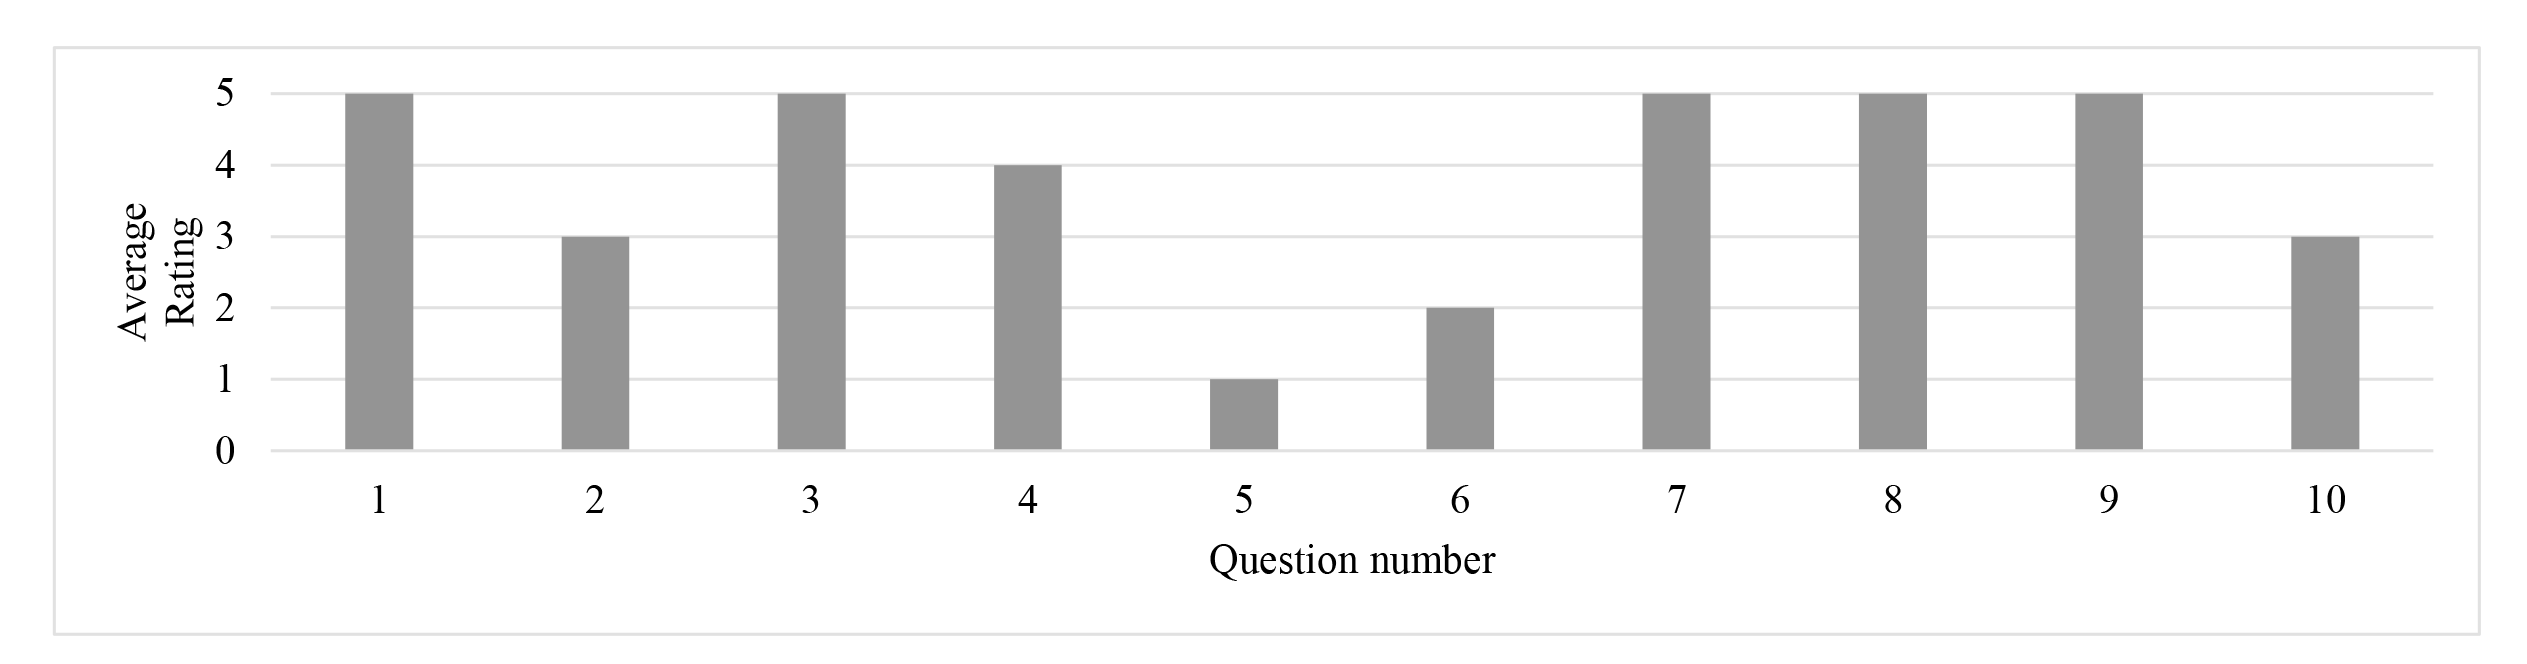
\includegraphics[width=1\textwidth]{figures/task3.png}
    \caption{Task 3 Post-Questionnaire Responses.}
    \label{fig:task3}
\end{figure}

\subsubsection{Discussion}
The usability evaluation proved there were many positive aspects of the Quarters user interface. Every participant was able to complete their task, and in an efficient time, regardless of the browser or the device. The straightforward navigation of the application allowed the participants to navigate easily across the web application and communicate quickly, which is a high-level goal of the software. The questionnaire results showed that participants agreed that Quarters was easy and intuitive to use. Based on these usability results, one could infer that the design and implementation support Norman’s Design Principles, as discussed in the Detailed Design document. The participants of the usability test unanimously strongly agreed that they would use the Maintenance Ticketing, File Upload and Notifications features. After testing Quarters, in response to how frequently they would use Quarters, participants either did not change their mind, or said they would use it more frequently relative to what they had stated prior to testing Quarters. Several participants noted during the ‘talk-aloud’ that they could see Quarters solving a lot of issues they experience in their current households. These positive test results prove that Quarters has marketability. \\ \\
Quarters was not without its weaknesses though. Not every participant saw the value in using Quarters on a daily basis and not every participant would recommend Quarters to a friend. Additionally, Quarters performed poorly on questions 5 and 6, which tested the usability of the Chat feature and the Finances feature, respectively. Participants noted during the ‘talk-aloud’ that they could not see a use for the Chat feature when the Bulletin Board allowed them the same functionality. Additionally, they noted that the purpose of the Finances feature was not initially clear. One landlord noted that they saw value in the File Upload feature, but not so much in the other features. Lastly, some users with a keen eye for design noted some glitches or flaws in our interface. \\ \\
 



\subsection{Performance}
To load test our server, we used the free trial of Load Impact(loadimpact.com) to simulate 25 users making requests to the server simultaneously; result is shown in \ref{fig:loadTest}.
\\From the graph, you can see that the load time is fairly consistent as the number of users increase.

\begin{figure}[h]
    \centering
    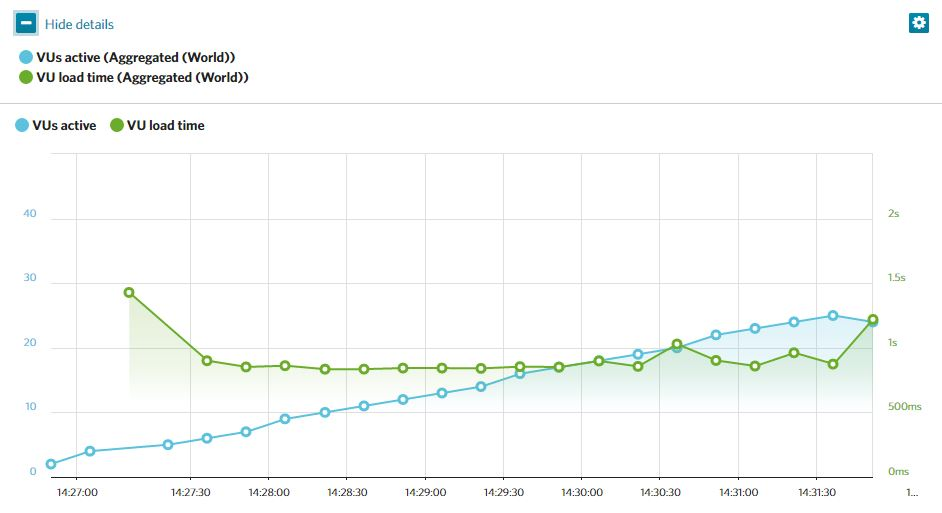
\includegraphics[width=1\textwidth]{figures/loadtest.JPG}
    \caption{Load Test result}
    \label{fig:loadTest}
\end{figure}


\subsection{Robustness}
Quarters application is tested against various browser and hardware devices to ensure that it will work in all environments.

\begin{longtable}{|L{2cm}|L{2cm}|L{5cm}|L{3.5cm}|L{1.5cm}|}
    \hline
    \textbf{Browser} & \textbf{Device} & \textbf{Look and feel} & \textbf{Functionalities} & \textbf{Bugs}\\
    \hline
    \textbf{Edge} & Computer & As expected & As expected & None \\
    \hline
    \multirow{3}{3em}{\textbf{Firefox}} & Computer & As expected & As expected & None \\
    \cline{2-5}
    & Android & As expected (Auto resize) & As expected & None \\
    \cline{2-5}
    & iOS & As expected (Auto resize) & As expected & None \\
    \hline
    \multirow{3}{3em}{\textbf{Chrome}} & Computer & As expected & As expected & None \\
    \cline{2-5}
    & Android & As expected (Auto resize) & As expected & None \\
    \cline{2-5}
    & iOS & As expected (Auto resize) & As expected & None \\
    \hline
    \multirow{3}{3em}{\textbf{Opera}} & Computer & As expected & As expected & None \\
    \cline{2-5}
    & Android & As expected (Auto resize) & As expected & None \\
    \cline{2-5}
    & iOS & As expected (Auto resize) & As expected & None \\
    \hline
    \multirow{2}{3em}{\textbf{Safari}} & Computer & As expected & As expected & None \\
    \cline{2-5}
    & iOS & As expected (Auto resize) & As expected & None \\
    \hline
\end{longtable}

\textbf{Permission}: When the user logs in and select a house, he is assigned a role(admin/member), each role has different permissions, for example, only admin can invite new members into the house. In additional to having different roles, the user can only edit/delete ``contents'' owned by himself.\\

\textbf{Session time out}: Session timed out after 30 minutes of inactivity, in which the user is logged out.


\section{Summary of Changes}
Moving forward, there is room for improvement with regard to the non-functional tests. Removing the Chat feature is something to consider to ensure all of our features collectively integrate well into Quarters. Redesigning the Finances feature or adding more functionality to it may help users understand its purpose more intuitively. Devoting more time and focus to styling would help resolve any design concerns and give the interface a more polished and professional appearance. Hopefully, with these changes, more participants would consider using Quarters more frequently and recommending the application to a friend. The results of the usability test have low external validity; in future usability tests, it would be worthwhile to seek a more diverse testing population outside of a school setting, with more landlords participating. Furthermore, a more complex set of tasks for test participants could give a more accurate reading of the effectiveness and efficiency of our application.


\end{document}
